%%%%%%%% ICML 2020 EXAMPLE LATEX SUBMISSION FILE %%%%%%%%%%%%%%%%%

\documentclass{article}

% Recommended, but optional, packages for figures and better typesetting:
\usepackage{microtype}
\usepackage{graphicx}
\usepackage{subfigure}
\usepackage{booktabs} % for professional tables

\usepackage{amsmath}
\usepackage{textcomp}
\usepackage{amssymb}

% hyperref makes hyperlinks in the resulting PDF.
% If your build breaks (sometimes temporarily if a hyperlink spans a page)
% please comment out the following usepackage line and replace
% \usepackage{icml2020} with \usepackage[nohyperref]{icml2020} above.
\usepackage{hyperref}

% Attempt to make hyperref and algorithmic work together better:
\newcommand{\theHalgorithm}{\arabic{algorithm}}

% Use the following line for the initial blind version submitted for review:
\graphicspath{{figs/}}
\usepackage[accepted]{src/icml2020}

% If accepted, instead use the following line for the camera-ready submission:
%\usepackage[accepted]{icml2020}

% The \icmltitle you define below is probably too long as a header.
% Therefore, a short form for the running title is supplied here:

\icmltitlerunning{Lifelong Control of Off-grid Microgrid with Model-Based Reinforcement Learning}

\newcommand{\ubar}[1]{\text{\b{$#1$}}}
% Community price
\newcommand{\lowPriceCom}{\ensuremath{y^\text{com, low}}}
\newcommand{\highPriceCom}{\ensuremath{y^\text{com, high}}}
\newcommand{\impCom}[1]{\ensuremath{i^\text{com, #1}}}
\newcommand{\expCom}[1]{\ensuremath{e^\text{com, #1}}}
\newcommand{\maxImpCom}{\ensuremath{\overline{I}^\text{com}}}
\newcommand{\maxExpCom}{\ensuremath{\overline{E}^\text{com}}}
\newcommand{\expGridB}{\ensuremath{y^\text{grid, exp}}}
\newcommand{\impGridB}{\ensuremath{y^\text{grid, imp}}}
\newcommand{\expComB}{\ensuremath{y^\text{com, exp}}}
\newcommand{\impComB}{\ensuremath{y^\text{com, imp}}}

% Battery
\newcommand{\BSSs}{\ensuremath{\mathcal{B}}}
\newcommand{\OPSOC}{\ensuremath{s}}
\newcommand{\maxcharge}{\ensuremath{\overline{S}}}
\newcommand{\mincharge}{\ensuremath{\underline{S}}}
\newcommand{\chargerate}{\ensuremath{\overline{P}}}
\newcommand{\dischargerate}{\ensuremath{\underline{P}}}
\newcommand{\retentionRate}{\ensuremath{\eta^{\text{retention}}}}
\newcommand{\chargeEfficienty}{\ensuremath{\eta^{\text{charge}}}}
\newcommand{\dischargeEfficienty}{\ensuremath{\eta^{\text{discharge}}}}
\newcommand{\initialCharge}{\ensuremath{S^\text{init}}}
\newcommand{\minEndCharge}{\ensuremath{\underline{S}^\text{end}}}
\newcommand{\maxEndCharge}{\ensuremath{\overline{S}^\text{end}}}
\newcommand{\charge}{\ensuremath{P^{\text{charge}}}}
\newcommand{\discharge}{\ensuremath{P^{\text{discharge}}}}

% Devices
\newcommand{\devices}[1]{\ensuremath{\mathcal{P}^\text{#1}}}
\newcommand{\sheddableDevices}{\ensuremath{\devices{sheddable}}}
\newcommand{\flexibleDevices}{\ensuremath{\devices{flexible}}}
\newcommand{\nonflexibleDevices}{\ensuremath{\devices{non-flexible}}}
\newcommand{\steerableDevices}{\ensuremath{\devices{steer}}}
\newcommand{\nonsteerableDevices}{\ensuremath{\devices{non-steer}}}
\newcommand{\assistBatteries}{\ensuremath{\BSSs^\text{assist}}}
\newcommand{\noassistBatteries}{\ensuremath{\BSSs^\text{no assist}}}

\newcommand{\Batteries}{\ensuremath{\BSSs}}
\newcommand{\Discharge}{\ensuremath{p^{discharge}}}
\newcommand{\Charge}{\ensuremath{p^{charge}}}

% Users
\newcommand{\users}{\ensuremath{\mathcal{U}}}
\newcommand{\profit}[1]{\ensuremath{c^\text{#1}}}
\newcommand{\optprofit}[1]{\ensuremath{J^{\star, \text{#1}}}}
\newcommand{\profitshare}[2]{\ensuremath{r^{#1}(J^{\star, \text{MU}}, #2)}}
\newcommand{\netEntityPosition}{\ensuremath{p}^{\text{net}}}

% Power assist
\newcommand{\maxImport}{\ensuremath{I}^{\text{max}}}
\newcommand{\maxExport}{\ensuremath{E}^{\text{max}}}
\newcommand{\assistanceOn}{\ensuremath{y}^{\text{assist}}}
\newcommand{\assistLevel}{\ensuremath{z}^{\text{assist}}}
\newcommand{\assistedPower}{\ensuremath{p}^{\text{assisted}}}
\newcommand{\assistlevel}{\ensuremath{P}^{\text{assist}}}
\newcommand{\netPositionUB}{\ensuremath{p}^{\text{net, UB}}}


% Dual variables
\newcommand{\dualSU}[1]{\ensuremath{\lambda^\text{#1}}}
\newcommand{\dualMU}[1]{\ensuremath{\beta^\text{#1}}}

% operator
\newcommand{\operatorincome}{\ensuremath{J}^\text{operator}}

% Peak power
\newcommand{\peak}{\ensuremath{\overline{p}}}
\newcommand{\oldpeak}{\ensuremath{\overline{p}^{\text{past}}}}
\newcommand{\peakdiscount}{\ensuremath{\gamma}^{\text{peak}}}
\newcommand{\peakincrease}{\ensuremath{\delta \overline{p}}}

% Price
\newcommand{\OPprice}[1]{\ensuremath{\pi^{\text{#1}}}}

% Cost
\newcommand{\OPcost}[1]{\ensuremath{c^\text{#1}}}

% Energy
\newcommand{\exportGrid}{\ensuremath{e}^\text{grid}}
\newcommand{\OPimport}{\ensuremath{i}^\text{grid}}
\newcommand{\exportSlack}{\ensuremath{e}^\text{slack}}
\newcommand{\importSlack}{\ensuremath{i}^\text{slack}}
\newcommand{\OPexchangeOut}{\ensuremath{e}^\text{com}}
\newcommand{\OPexchangeIn}{\ensuremath{i}^\text{com}}
\newcommand{\OPprod}{\ensuremath{p^{\text{prod}}}}
\newcommand{\OPcons}{\ensuremath{p^{\text{cons}}}}

% Reserve
\newcommand{\OPreserve}[1]{\ensuremath{r^\text{#1}}}

% Time
\newcommand{\OPduration}{\ensuremath{\Delta_t}}
\newcommand{\OPperiods}{\ensuremath{\mathcal{T}}}

%Production
\newcommand{\curtail} {\ensuremath{P^\text{curt}}}
\newcommand{\steer}{\ensuremath{P^\text{steer}}}
\newcommand{\nonSteerable}{\ensuremath{P^\text{non-steer}}}
\newcommand{\steerable}{\ensuremath{P^\text{steer}}}

% Consumption
\newcommand{\shed} {\ensuremath{C^\text{shed}}}
\newcommand{\flex}{\ensuremath{C^\text{flex}}}
\newcommand{\flexCons}{\ensuremath{c^\text{flex}}}
\newcommand{\flexStart}{\ensuremath{y^\text{flex}}}
\newcommand{\flexStarted}{\ensuremath{z^\text{flex}}}
\newcommand{\exclusiveGroup}{\ensuremath{\mathcal{G}}}
\newcommand{\nonFlexible}{\ensuremath{C^\text{non-flexible}}}
\newcommand{\flexibleLoadDuration}{\ensuremath{\text{duration}^\text{flex}}}
\newcommand{\flexibleLoadProfile}{\ensuremath{\text{profile}^\text{flex}}}
\newcommand{\flexibleLoadStartTime}{\ensuremath{\text{start}^\text{flex}}}
\newcommand{\flexibleLoadEndTime}{\ensuremath{\text{end}^\text{flex}}}
\newcommand{\flexibleLoadAcceptanceRatio}{\ensuremath{\underline{a}^\text{flex}}}
\newcommand{\flexibleLoadMustRun}{\ensuremath{\text{run}^\text{flex}}}
\newcommand{\flexibleEnergy}{\ensuremath{\text{E}^\text{flex}}}
\newcommand{\sheddable}{\ensuremath{C^\text{sheddable}}}
\newcommand{\maxSheddingTime}{\ensuremath{\overline{t}^\text{shedding}}}

% Sharing
\newcommand{\weight}[1]{\ensuremath{w^\text{#1}}}

% Misc 
\newcommand{\forallt}{\ensuremath{\forall t \in \OPperiods}}
\newcommand{\forallu}{\ensuremath{\forall u \in \users}}

\begin{document}

\twocolumn[
\icmltitle{Lifelong Control of Off-grid Microgrid with Model-Based Reinforcement Learning}

% It is OKAY to include author information, even for blind
% submissions: the style file will automatically remove it for you
% unless you've provided the [accepted] option to the icml2020
% package.

% List of affiliations: The first argument should be a (short)
% identifier you will use later to specify author affiliations
% Academic affiliations should list Department, University, City, Region, Country
% Industry affiliations should list Company, City, Region, Country

% You can specify symbols, otherwise they are numbered in order.
% Ideally, you should not use this facility. Affiliations will be numbered
% in order of appearance and this is the preferred way.
\icmlsetsymbol{equal}{*}

\begin{icmlauthorlist}
\icmlauthor{Simone Totaro}{equal,upf}
\icmlauthor{Ioannis Boukas}{equal,be}
\icmlauthor{Anders Jonsson}{upf}
\icmlauthor{Bertrand Corn\'elusse}{be}
\end{icmlauthorlist}

\icmlaffiliation{upf}{Department of Information and Communication Technologies\\ Universitat Pompeu Fabra, Barcelona, Spain.}%\\ Email: \{simone.totaro, anders.jonsson\}@upf.edu}

\icmlaffiliation{be}{Department of Electrical Engineering and Computer Science, University of Li\`ege, Li\`ege, Belgium.} %% Email: \{ioannis.boukas, bertrand.cornelusse\}@uliege.be}

\icmlcorrespondingauthor{Ioannis Boukas}{ioannis.boukas@uliege.be} % ale?

% You may provide any keywords that you
% find helpful for describing your paper; these are used to populate
% the "keywords" metadata in the PDF but will not be shown in the document
\icmlkeywords{Microgrid control, optimization, reinforcement learning, Dyna.}

\vskip 0.3in
]

% this must go after the closing bracket ] following \twocolumn[ ...

% This command actually creates the footnote in the first column
% listing the affiliations and the copyright notice.
% The command takes one argument, which is text to display at the start of the footnote.
% The \icmlEqualContribution command is standard text for equal contribution.
% Remove it (just {}) if you do not need this facility.

%\printAffiliationsAndNotice{} % leave blank if no need to mention equal contribution
\printAffiliationsAndNotice{\icmlEqualContribution} % otherwise use the standard text.

\begin{abstract}
    \textcolor{black}{Off-grid microgrids are receiving a growing interest for rural electrification purposes in developing countries due to their ability to ensure affordable, sustainable and reliable energy services. Off-grid microgrids rely on renewable energy sources (RES) coupled with storage systems to supply the electrical consumption. The inherent uncertainty introduced by RES as well as the stochastic nature of the electrical demand in rural contexts pose significant challenges to the efficient control of off-grid microgrids throughout their entire life span.} In this paper, we address the lifelong control problem of an isolated microgrid. We categorize the set of changes that may occur over its life span in progressive and abrupt changes. We propose a novel model-based reinforcement learning algorithm that is able to address both types of changes. In particular, the proposed algorithm demonstrates generalisation properties, transfer capabilities and better robustness in case of fast-changing system dynamics. The proposed algorithm is compared against a rule-based policy and a model predictive controller with look-ahead. The results show that the trained agent is able to outperform both benchmarks in the lifelong setting where the system dynamics are changing over time.
\end{abstract}

\section{ Introduction} \label{sec: Introduction}
	Microgrids are small electrical networks composed of flexible consumption, distributed power generation (renewable and/or conventional) and storage devices. The operation of a microgrid is optimized in order to satisfy the demand while ensuring maximum reliability and power quality and to maximize the renewable energy harvested locally while minimizing the total system cost.

	Centralized microgrid control is usually decomposed in four tasks: i) estimating the parameters of the microgrid devices (for instance the charge efficiency of a battery storage device as a function of the state of charge and temperature, or the actual capacity of a battery after a number of cycles), ii) forecasting the consumption and the renewable production, iii) operational planning to anticipate weather effects and human activities, and iv) real-time control to adapt planned decisions to the current situation. These tasks are preformed sequentially during the lifetime of a microgrid in order to achieve near optimal operation and to maximize the benefits arising from distributed generation. 

	After the initial parameters' estimation step, it is important for the efficient microgrid operation to incorporate in the decision making process all the sources of uncertainty. To this end, forecasting techniques are deployed for the stochastic production and consumption. There is a variety of forecasting techniques in the literature ranging from fundamental models of consumption and renewable energy production \cite{Dolara2015} to statistical models using measured data \cite{Lombardi2019}. 

	Subsequently, the outputs of the forecasting models in combination with the system parameters are used to compute the optimal control actions that need to be taken. The optimization of the control actions can be performed using the simulation model of the microgrid. Model predictive control (MPC), a feedback control law meant to compensate for the realization of uncertainty, is often used for achieving economic efficiency in microgrid operation management \cite{Parisio2014}. \textcolor{black}{Probabilistic forecasting models attempt not only to provide the best point forecast but instead target the distribution of the uncertainty. The output of these models can be used to solve stochastic variants of MPC \cite{BRUNI2016119}. Depending on the reliability concerns related to the micorgrid use case, robust MPC can provide more secure ways of dealing with uncertainty \cite{ZHANG20181229}.} Given the data availability, the two preceding tasks, namely forecasting and optimization, can be merged into one task and a control action can be derived directly from the data observed. 
    
    
	In this paper, we present an open-source reinforcement framework for the modeling of an off-grid microgrid for rural electrification. Moreover, we formulate the control problem of an isolated microgrid as a Markov Decision Process (MDP). Due to the high-dimensional continuous action space we define a set of discrete meta-actions in a similar way to previous work~\cite{Boukas2018}.

	The main challenge for the lifelong control of an off-grid microgrid arises from the uncertainty of the future renewable production and consumption. A critical issue in microgrid operation is that often-times the policy learned during training on a dataset does not perform well on unseen data. Additionally, the degradation or damage of the various components such as the storage devices or the photovoltaic panels cause the previously learned policies to become sub-optimal over time.

	\textcolor{black}{To address these challenges we propose a novel model-based reinforcement learning algorithm. In particular, this class of algorithms integrates planning and learning of an optimal control. They do so by firstly estimating a model of the environment from samples collected by interactions with the environment and by subsequently using this model to generate synthetic trajectories that accelerate the learning process of the control policy. The motivation for learning the dynamics of the environment stems from the enhanced exploration that yields generalization and transferability properties that are highly desired in the context where changes are introduced in the environment.}
	
	In particular, the proposed algorithm is an instance of \textsc{Dyna} \cite{sutton2012dyna}, where the model is trained using distributional losses and the policy is optimized using the Proximal Policy Optimization (PPO) algorithm. \textcolor{black}{A comprehensive description of the algorithms mentioned can be found in Sections \ref{sec:dyna} and \ref{sec:PPO}}. The values of the policy are updated based on the expectation computed over a set of states sampled from a model. This model is trained online using samples from the real environment. We illustrate that this algorithm allows for much better estimation of the values accounting for the uncertainties and yields enhanced exploration. Additionally, we show that the enhanced exploration gained using the model to sample states allows for better generalization to unseen data. Moreover, we show that the knowledge of a previously trained policy can be efficiently transferred when training on a new set of data. Finally, we demonstrate the ability of the controller to adapt to sudden changes such as damage of the equipment without explicit knowledge of the event. 

	A key advantage of the model-based approach is that it can help cope with rare events, in case those rare events have been experienced at least once before in the past. Since \textsc{Dyna} builds a model of the dynamics and simulates transitions using the learned model, it can repeat rare events many times in simulation and update the policy accordingly. The disadvantage is that the non-stationary time series of consumption and renewable production are difficult to predict, and that quantile regression may cause approximation errors.

	To evaluate the performance of the obtained policy, we compare it with two benchmarks: i) a rule-based control that takes decisions in a myopic manner based only on current information; and ii) an optimization-based controller in which look-ahead is applied to forecast consumption and RES generation.

	This paper is organized as follows. Section~\ref{sec: RelatedWork} elaborates on state-of-the-art methods used for data-driven microgrid operation and control.  In Section~\ref{sec: Simulator}, the system dynamics of the microgrid are detailed. Section~\ref{sec: RLBackground} provides the theoretical background used for the developed framework and the algorithm proposed. In Section~\ref{sec: ProblemStatement}, we formulate the lifelong control problem of an off-grid microgrid as an MDP. Section~\ref{sec: Algorithm} presents the model-based algorithm used to solve the lifelong microgrid control problem. The proposed algorithm is compared against the two benchmark strategies presented in Section~\ref{sec: Bechmarks}. Section~\ref{sec: CaseStudy} describes the case study and results obtained. Finally, Section~\ref{sec: conclusions} concludes the main findings and provides avenues for future research.

\section{Related Work and Contributions} \label{sec: RelatedWork}

	\textcolor{black}{A wide range of reinforcement learning techniques have been applied in the literature for optimizing energy systems operations. A vast share of these techniques include model-free reinforcement learning algorithms, where a controller is trained based solely on interactions with the physical environment and without using prior knowledge regarding system dynamics. For instance, the problem of controlling a storage device connected to the main grid in order to maximize its returns and to facilitate RES integration is proposed in \cite{lee2012intelligent}. A bias correction procedure of the classical Q-learning algorithm \cite{watkins1992q} was proposed and the results show a much faster and more stable converge than the vanilla version of the algorithm.
	The efficient storage control aiming at jointly mazimizing the usage of the battery during high electricity demand and the RES utilization in a grid connected microgrid setting is proposed in \cite{Kuznetsova2013}. Predictions about the wind generation serve as input to a reinforcement learning controller that is responsible for the battery scheduling. In particular, the optimal control policy is computed using the Q-learning method. \textcolor{blue}{In both settings the state and action spaces are discretized in order to reduce the computational complexity and the results show an average increase in the utilization of renewable energy sources (RES) that amounts to approximately 10\%}. However, this reduction of complexity inherently puts a limit to the performance improvement margins.} 
	
	\textcolor{black}{Alternatively, the energy management of a grid-connected microgrid can be performed in a distributed way. Each entity of the microgrid that owns equipment (e.g. PV panels, storage etc.) acts as an autonomous agent who can learn the best response policy to increase their expected rewards in a microgrid market though interaction with other agents \cite{foruzan2018reinforcement}. Reinforcement learning is used as a method to develop optimal strategies for energy management and the authors show that the proposed game converges to the Nash equilibrium. A similar multi-agent setting is adopted in \cite{KOFINAS201853} where the authors propose a fuzzy Q-Learning method to solve the control problem in a decentralized manner. Each component (i.e. storage, load, PV panels) act as independent learners and a common information state is shared between them in order to coordinate their behavior. \textcolor{blue}{Results show that adopting this decentralized coordinated control approach leads to increased reliability and enhanced  guarantees of energy supply i.e. the uncovered energy is very low and corresponds to 1.54\% of the total demand.} However, a centralized approach is more relevant in the context of rural electrification and generally leads to more tractable problems. In this paper, we consider a central entity that owns an energy management system (EMS) and is making the control decisions over the controllable components.}
	
	\textcolor{black}{Recent advancements in the field of Deep Learning (DL) have enabled the use of powerful function approximation techniques for representing value functions and policies that can support (as input/output) continuous and high dimensional state/action spaces. For instance,  Q-learning combined with Artificial Neural Networks has been proposed for the optimal operation and maintenance of power grid \cite{ROCCHETTA2019291}, which is inherently a very large and complex problem. The proposed framework outperforms expert-based solutions to grid operation. Leveraging these techniques, researchers have also proposed a Deep Q-learning approach for the control of seasonal storage in an isolated microgrid~\cite{franccois2016deep}. In this framework, a specific deep learning structure is presented in order to extract information from the past RES production and consumption as well as the available forecasts. Despite the highly dimensional continuous state space, the authors obtain a control policy that is able to utilize the long-term storage in a meaningful way. However, in this approach it is assumed that the dynamics of the system are linear and that forecasts of the variable resources are available.}
	
	\textcolor{black}{As it is shown, model-free reinforcement learning methods are able to tackle quite well the energy management problem in contexts (environments) where the dynamics remain unchanged. However, in this paper we consider an environment in which changes (gradual and abrupt) are expected to occur during the operational horizon of the microgrid. To tackle this problem, we resort to model-based reinforcement learning, where a model of the system dynamics is learnt by interaction with the environment and then used for taking control actions. Model-based methods have shown better performance in terms of enhanced exploration \cite{lopes2012exploration}, accelerated learning \cite{kaiser2019model} and have proven to be suitable in real world non-stationary environments \cite{lopes2012exploration, polydoros2017survey}.
	}
	
	In this direction, in \cite{shuai2020line}, the energy scheduling in a residential microgrid is performed by adapting \textit{MuZero} \cite{schrittwieser2019mastering}, a state of the art model-based reinforcement learning algorithm, to the problem. It incorporates the learning of a complex model that is then used for performing Monte-Carlo tree search (MCTS) for the selection of the optimal action. However, the MCTS algorithm relies heavily on the accuracy of the learnt model for simulating several steps in the future. In the context of a changing environment, this approach could lead to sub-optimalities driven by the increasing inaccuracy of the learnt model as the prediction length increases. \textcolor{black}{Additionally, the search for the next action is performed online given some computational budget which might raise reliability issues. In the approach presented in this paper, the training of the policy is assisted by a model of the system dynamics and it is performed off-line. The trained policy is then used in real time for dispatching the microgrid components.}
	
	\textcolor{black}{
	 The use of model-based reinforcement learning with Power Pinch Analysis (PoPA) has proven to be an effective way to coordinate several storage technologies with complementary features in order to enhance the reliability of intermittent renewable energy sources (RES) \cite{NYONGBASSEY2020116622}. In particular, the authors propose an adaptive version of PoPA where \textsc{Dyna-Q} \cite{SUTTON1990216} is used to account for the variability introduced by RES and the demand. A physical model is used together with the RES predictions to simulate the future evolution of the system. Corrective actions are taken in order to avoid the violation of upper and lower limits set. In this paper, we do not consider a physical model of the system. Instead, we attempt to learn an approximation (neural network) of the system dynamics based on simulated experience. In this way, any changes that might occur in the environment can be learnt through demonstration.}
	
	\textcolor{black}{The contributions of this paper are the following:
	\begin{itemize}
	    \item We present an open-source reinforcement learning framework for the lifelong modeling of an off-grid microgrid for rural electrification. Any changes (gradual/abrupt) that may occur over the lifetime of the microgrid are incorporated in this framework.
	    \item We propose a novel model-based reinforcement learning algorithm, where the model of the system is trained using quantile regression and the PPO algorithm is used for training the policy.
	    \item The proposed algorithm is evaluated by its ability to perform well in changing conditions. To this end, we demonstrate that the algorithm is able to outperform the benchmark control algorithms in i) a setting where the electricity consumption is changing progressively and ii) a setting where a sudden failure of the storage device occurs.
	\end{itemize}
	}

\section{Microgrid Description}\label{sec: Simulator}
    \label{sec:gym}
    % find another notation !!!
    \textcolor{black}{In this section, we provide a detailed description of the system considered (Figure \ref{fig:MG}). The considered microgrid is composed of PV panels, a diesel generator, a battery and aims at providing energy to variable loads. The Energy Management System (EMS) is responsible for the interaction and the scheduling of the controllable components. As depicted in Figure \ref{fig:MG}, the EMS receives as inputs information about the production from the pv panels and the load consumption. Subsequently, the role of the EMS is to decide on whether to activate the diesel generator and/or to discharge/charge the battery. In the following we provide a detailed description of the components considered. Additionally, an off-grid microgrid designed for rural electrification is inherently characterized by changes occurring in different time-scales. We provide a formal description of the different types of changes and we motivate the need for a lifelong control that has the ability to adapt to these changes.}
    
    \begin{figure}[h!]
	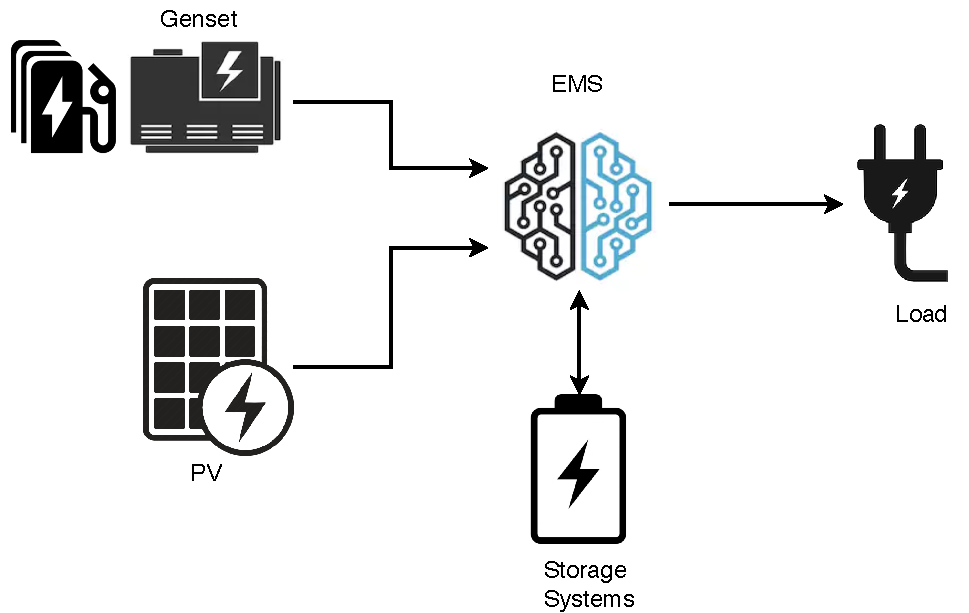
\includegraphics[width=0.5\textwidth]{microg.pdf}
	\centering
	\caption{Schematic of the considered microgrid.}
	\label{fig:MG}
    \end{figure}
    
\subsection{Components}

An off-grid microgrid is composed of the following components:
 
\subsubsection{Consumption} 
    
    The consumption of the isolated microgrid $\nonFlexible$ is considered to be non-flexible, meaning that there is a high cost associated to the energy non-served. The consumption $\nonFlexible_{t}$ at each time-step $t$ of the simulation is assumed to be a stochastic variable that is sampled from distribution $P^{C}_{t}$, given the $h$ previous realizations, according to:
    \begin{gather}
    \nonFlexible_{t} \sim P^{C}_{t}( \nonFlexible_{t-1}, ...,\nonFlexible_{t-h} ).\label{eqn: load}
    \end{gather}
    In this paper, it is represented by real data gathered from an off-grid microgrid. The distribution $P^{C}_{t}$ is indexed in time in order to indicate that changes occur in the aggregate consumption over the life-time of the microgrid. For instance, a change in the consumption profile can be caused by the fact that more users are progressively connected to the micro-grid.

\subsubsection{Storage model}
    
    The modeling of the storage system can become quite complex and highly-nonlinear depending on the degree of accuracy required by each specific application. In this paper, we use a linear ``tank'' model for the simulation of the battery since we assume that the simulation time-step size $\Delta t$ is large enough (1 hour). The dynamics of a battery are given by:
    \begin{gather}
    SoC_{t+1} = SoC_{t}+ \Delta t\cdot(\chargeEfficienty \charge_t - \frac{\discharge_t}{\dischargeEfficienty}) ,\label{eqn: storagedynamics}
    \end{gather}
    where $SoC_{t}$ denotes the state of charge at each time step $t$, $\charge$ and $\discharge$ correspond to the charging and discharging power, respectively and $\chargeEfficienty$, $\dischargeEfficienty$ represent the charging and discharging efficiencies of the storage system. The charging ($\charge$) and discharging ($\discharge$) power of the battery are assumed to be limited by a maximum charging rate $\chargerate$ and discharging rate $\dischargerate$, respectively. Accounting for the storage system degradation, we consider that the maximum capacity $\maxcharge$ of the storage system as well as the charging and discharging efficiencies ($\chargeEfficienty$, $\dischargeEfficienty$) are decreasing as a linear function of the number of cycles $n_t$ that are performed at each time-step $t$. We have, $\forall t \in T$, 
    \begin{align}
    SoC_{t}, \charge_t, \discharge_t &\geq 0 \\
    \charge_t &\leq \chargerate\\
    \discharge_t &\leq \dischargerate , \\
    SoC_{t} &\leq \maxcharge \label{eqn: storage limits},\\
    \maxcharge&=s(n_t). \label{eqn: storage_limits_evolving}
    \end{align}
    

\subsubsection{Steerable generator model}
    Steerable generation is considered any type of conventional fossil-fuel-based generation that can be dispatched at any time-step $t$. When a generator is activated, it is assumed to operate at the output level $\steer_t$ that is ranging between the minimum stable generation $\underline{\steerable}$ and the maximum capacity $\overline{\steerable}$ such that:
    \begin{gather}
    \underline{\steerable} \leq \steer_t \leq \overline{\steerable}.\label{eqn: generatordynamics}
    \end{gather}
    The fuel consumption $F_t$ related to the operation of the generator at time $t$ is a function of the power output $\steer_t$ with parameters $F_1$, $F_2$ given by the manufacturer. 
    \begin{gather}
    \begin{split}
    F_t =  
    \begin{cases}
    F_1 + F_2 \cdot \steer_t &, \text{if } \steer_t>0,   \\
    0  &, \text{otherwise}.
    \end{cases}
    \end{split}.\label{eqn: fuelconsuption}
    \end{gather}
    
    
    The fuel cost $\OPcost{fuel}_t$ accounting for the fuel price $\OPprice{steer}$ is then given by:
    \begin{gather}
    \OPcost{fuel}_t = F_t \cdot \OPprice{fuel} .\label{eqn: generatorcost}
    \end{gather}
    
\subsubsection{Non-steerable generators model}
    The level of non-steerable generation from renewable resources such as wind or solar is denoted by $\nonSteerable$. Similar to the non-flexible load case it is assumed that $\nonSteerable_t$ at time-step $t$ is sampled from a probability distribution $P^{\nonSteerable}_{t}$, given the $h$ previous realizations, according to:
    \begin{gather}
    \nonSteerable_t \sim P^{\nonSteerable}_{t}( \nonSteerable_{t-1},...,\nonSteerable_{t-h}).\label{eqn: pv}
    \end{gather}
    In this paper, the renewable generation is represented by real data gathered from an off-grid microgrid. Similar to the case of the non-flexible load, the distribution $P^{\nonSteerable}_{t}$ is indexed by time $t$ to indicate that changes in the renewable production might occur over time. These changes are mostly related to the progressive degradation of the equipment (solar panels).
    
\subsubsection{Power balance}
    At each time-step $t$ in the simulation horizon we compute the power balance between the injections and the off-takes. The residual power resulting from the mismatch between production and consumption is curtailed $\curtail_t$ if its positive and shed $\shed_t$ if it is negative. We can formally define the power balance as:
    \begin{gather}
    \nonSteerable_{t} + \steer_{t} + \discharge_{t} + \shed_{t} \\\notag
    =\charge_{t} + \curtail_{t}  + \nonFlexible_{t},\label{eqn: powerbalance}
    \end{gather}
    with $\curtail_t , \shed_t \geq 0$.
    The costs arising from the curtailment of generation or the shedding of non-flexible loads are given by: 
    \begin{gather}
    \OPcost{curt}_t = \curtail_t \cdot \OPprice{curt} \label{eqn: curtcost}\\
    \OPcost{shed}_t = \shed_t \cdot \OPprice{shed} \label{eqn: shedcost}
    \end{gather}
    

\subsection{Characterizing changes in the environment}
	
	Oftentimes in real-life applications the concept of interest depends on some underlying context that is not fully observable. Changes in this underlying concept might induce more or less radical changes in the concept of interest, which is formally known as concept drift \cite{tsymbal2004problem}. For instance, in the off-grid microgrid under study the connection of new users and their habits have strong influence on distribution $ P^{C}_{t}$. However, it is not possible to know exactly and to quantify the effect on the consumption a priori. 
	
%	The extent of the drift is defined as the rate of change of the underlying distribution in two subsequent time instances and it is used to characterize the concept drift. Let $P_{t}$ be the underlying probability distribution. Computing the extent of the drift essentially boils down to computing the difference between two distributions using a norm (e.g. L1) $D(P_{t+1}||P_{t})$.

	In this paper, we deal with the following two distinct set of changes: 1) gradual changes that affect the non-controllable dynamics; and 2) sudden changes that affect the deterministic dynamics.
	As described in Section~\ref{sec: ProblemStatement}, one can decouple the two components of the state space. Gradual changes occurs in the stochastic component of the state space (\ref{eqn: stochastic_probabilities}) while sudden changes occurs in the deterministic system dynamics (\ref{eqn: transitionfunction}).
	
	
	%More formally, note that $P_t$ be the transition kernel defined in section \ref{sec: mdp} can be written as the composition of the system dynamics $f_t(a_t, \bar{s}_t)$ and the non controllable stochastic process $F_t(\ubar{s}_t)$.

	\subsubsection{Gradual changes}
	These are cases in which a slow concept drift occurs. The extent of the drift is bounded so that any learner can follow these changes successfully. A formal bound on the maximal rate of drift that is acceptable by a batch-based learner is given by \citet{kuh1991learning}. In this paper, we assume that changes related to the consumption and renewable production profiles as well as degradation of the equipment (storage) belong to this category.
	
	\subsubsection{Sudden or abrupt changes}
	In our setting, sudden or abrupt changes are adversarial changes that affect the system dynamics, and for which the learner needs to find the best response. Robust MDPs \cite{nilim2005robust} describe optimal control under such changes and recent work \cite{lim2013reinforcement} shows that incorporating learning in such contexts can deliver policies as good as the minimax policy. \citet{gajane2018ucrl} also propose an algorithm for detecting abrupt changes in MDPs. In the concept of an off-grid micro-grid this type of change would typically occur during equipment failure. \textcolor{black}{In the case study presented in Section \ref{sec: robustness}, we consider a sudden failure of the storage system. This event leads to a sudden change in the optimal control policy where the generator becomes the main source of power when the RES are not producing sufficiently. Another example of an abrupt change could be the sudden connection of a large industrial consumer to the microgrid. This would have a significant and direct impact to the control policy as well.} 

\section{Reinforcement Learning Background} \label{sec: RLBackground}
    \textcolor{black}{In this section, we provide the theoretical background used for the developed framework and the proposed methodology. We first introduce the Markov Decision Process that is the main framework on which we rely on for modeling the decision making process of an off-grid microgrid operator. We proceed by describing Dyna and Proximal Policy Optimization (PPO), which are the foundations of the proposed novel algorithm.}
    
\subsection{ Markov Decision Process}

    We consider an infinite horizon discounted Markov Decision Process (MDP), defined by the tuple $\langle S,A,r,\{P_t\}_t,\gamma \rangle$ where  $S$ is the state space, $A$ the action space, $r:S \times A \rightarrow \mathbb{R}$ is the Markovian cost function, $P_t: S \times A \rightarrow \Delta(S) $, $t\geq 0$, is the transition kernel at time $t$ and $\gamma \in (0, 1) $ is the discount factor. Here, $\Delta(S)$ is the probability simplex on $S$, i.e.~the set of all probability distributions over $S$. At each time step $t$, the agent observes state $s_t \in S$, takes an action $a_t \in A$, obtains reward $r_t$ with expected value $\mathbb{E}[r_t] = r(s_t, a_t)$, and transitions to a new state $s_{t+1} \sim P_t(\cdot \rvert s_t, a_t)$. We refer to $(s_t,a_t,r_t,s_{t+1})$ as a {\em transition}. Note that the transition kernels may not be stationary.
   
    Let $\pi$ denote a stochastic policy $\pi : S \rightarrow \Delta(A)$ and $\eta(\pi)$ its expected discounted cumulative reward under some initial distribution $d_0\in\Delta(S)$ over states: %{\color{red} with respect to a starting state?}
    \begin{gather}
    \eta(\pi) = E_{s\sim d_0} [V^{\pi}(s)],\label{eqn: expected_cumulative_reward}
    \end{gather}
    
	\noindent
     where $\tau = \{(s_t,a_t, r_t)\}_{t \geq 0}$ is a trajectory, $p(\tau)$ is the probability distribution over trajectories,  %{\color{red} perhaps relate $p$ to $P_t$?}
     \begin{equation}
        p(\tau) = d_0(s_0) \prod_{t=0}^\infty P_t(s_{t+1} \rvert s_t, a_t) \pi(a_t \rvert s_t),
     \end{equation}{}
     
 	\noindent
    and the value function $V^\pi$ is defined for each state $s\in S$ as
    \begin{gather}
        V^{\pi}(s) = E_{p(\tau)}\left[ \left. \sum_{t=0}^{\infty} \gamma^t r_t(s_t,a_t) \right\vert s_0=s \right].
    \end{gather}

    The goal of the agent is to find a policy that maximizes the expected cumulative reward $\eta(\pi)$:
    \begin{gather}
    \eta^{*} = \max_{\pi} \eta(\pi),\label{eqn: optimalcost}\\
    \pi^{*} = \arg \max_{\pi} \eta(\pi).\label{eqn: optimalpolicy}
    \end{gather}

    %  update is a placeholder
    \begin{algorithm}[t]
    	\caption{\textsc{Dyna}}
    	\begin{algorithmic}[1]
    		\STATE \textbf{Inputs}: MDP $M$, integers $T$, $B$, $N$
			\STATE initialize policy $\pi_\theta$, model $M_\psi$
    		\FOR{$t=0$ \TO $T-1$}
    			\STATE $s \sim d_0$
    			\STATE $a \sim \pi_\theta(\cdot \rvert s)$
    			\STATE $s',r \sim M(s,a)$
				\STATE $\pi_\theta = \,$ \textsc{updatePolicy}$(s,a,r, s')$
    			\STATE $M_\psi = \,$ \textsc{updateModel}$(s,a,r, s')$
    			\IF{$t \geq B$}
        			\FOR{$n=0$ \TO $N-1$}
        				\STATE  $s \sim d_0$
        				\STATE  $a \sim \pi_\theta(\cdot \rvert s)$
        				\STATE $\hat{s}', \hat{r} \sim M_\psi(s,a)$
        				\STATE $\pi_\theta = \,$ \textsc{updatePolicy}$(s,a,\hat{r}, \hat{s}')$
        			\ENDFOR
        		\ENDIF
    		\ENDFOR
    	\end{algorithmic}
    	\label{algodyna}
    \end{algorithm}
    
\subsection{ Dyna}\label{sec:dyna}
    % this methodology
    \textsc{Dyna} \cite{sutton2012dyna} is a model-based reinforcement learning architecture that aims to integrate learning and planning. 
    It does so by performing online estimation of the transition kernel and reward function. Let $M_\psi = \langle P_\psi, r_\psi \rangle$ be a parametric model learned during training. Note that we estimate a single transition kernel $P_\psi$ even though the true kernel may not be stationary.%  {\color{red} do we really estimate one transition kernel per time step?}
    
	Algorithm~\ref{algodyna} outlines the \textsc{Dyna} algorithm in the parametric setting. 
    For every transition $(s,a,r,s')$ sampled from the environment $M$, we update the policy $\pi_\theta$ and parametric model $M_\psi$ via update functions described in Algorithms~\ref{update_policy} and \ref{update_model}. We remark that the policy update typically relies on a value function $V_\phi$. Additionally, the value function $V_\phi$ and the components of the parametric model $M_\psi$ are updated by minimizing a loss function.
 
    After the update step, we use the learned model to perform $N$ updates of the policy $\pi_\theta$, in the same way as one would using the true environment. At every step, we sample a state $s \sim d_0$, apply action $a \sim \pi_\theta( \cdot \rvert s) $ and query the parametric model $\hat{s}', \hat{r} \sim M_\psi(s,a)$. % {\color{red} how do you sample $s$? Do you not just follow a trajectory?}
    
    Note that there are two main differences during the planning phase. First, the transition $(s, a, \hat{r}, \hat{s}')$ comes from the parametric model, and second, there is no structure in the sampling process, therefore in such an update the agent can experience any possible one step transition, even ones that are hard to gather under the current policy.
    
    
\begin{algorithm}[t]
	\caption{\textsc{updatePolicy}}
	\begin{algorithmic}[1]
		\STATE \textbf{Input}: transition $(s,a,r,s')$
		\STATE  $V_\phi = \arg\min_{V_\varphi} L^V(V_\varphi)$
		\STATE  $\pi_\theta = \arg\max_{\pi_\varphi} \eta (\pi_\theta)$
	\end{algorithmic}
	\label{update_policy}
\end{algorithm}

\begin{algorithm}[t]
	\caption{\textsc{updateModel}}
	\begin{algorithmic}[1]
		\STATE \textbf{Input}: transition $(s,a,r,s')$
		\STATE  $P_\psi = \arg\min_{P_\varphi} L^P(P_\varphi)$
		\STATE  $r_\psi = \arg\min_{r_\varphi} L^r(r_\varphi)$
	\end{algorithmic}
	\label{update_model}
\end{algorithm}


\subsection{ Proximal Policy Optimization}\label{sec:PPO}
    
    The Proximal Policy Optimization (PPO) algorithm \cite{Schulman2017} belongs to the family of policy gradient methods and can be used with both discrete and continuous action spaces. In the vanilla actor-critic method \cite{sutton2000policy}, a stochastic policy $\pi_\theta$ with parameters $\theta$ is optimized towards the following regularized objective:
    
    \begin{gather}
        \eta(\pi_\theta)  = \mathbb{E}_{p(\tau)}\left\lbrace 
        \frac{\pi_\theta(a_t \rvert s_t)}{\pi_o(a_t \rvert s_t  )} \hat{A}_{\phi}(s_t,a_t)\right\rbrace  - \frac{1}{\beta}  
        D( \pi_\theta \rvert \rvert \pi_o) ,\label{eqn: regularized}
    \end{gather}

	\noindent
	where $\pi_o$ is the old policy, $\hat{A}_{\phi}(s_t,a_t)$ is an estimator of the advantage function, $D$ is a regularizer in the form of a Bregman divergence and $\beta$ is a learning rate.
    
	Since equation \eqref{eqn: regularized} is hard to optimize directly, the policy is repeatedly updated using stochastic gradient descent. Concretely, a gradient step is used to update of the parameters $\theta$ as
    \begin{gather}
    \theta_{new} = \theta + \alpha \nabla \hat{\eta}(\pi_{\theta}),\label{eqn: thetaupdatesgrad}
    \end{gather}
    
	\noindent
    where $\alpha$ is a step size and the regularized objective for the individual transition $(s,a,r,s')$ is estimated as
	\begin{gather}
        \hat{\eta}(\pi_\theta)  =  \frac{\pi_\theta(a \rvert s)}{\pi_o(a \rvert s )} \hat{A}_{\phi}(s,a)  - \frac{1}{\beta}  
        \sum_{a'} \pi_\theta(a'|s) \log \frac {\pi_\theta(a'|s)} {\pi_o(a'|s)}. \label{eqn: regularized2}
    \end{gather}

	An unbiased estimator of the advantage function is given by 
    \begin{equation}
    \hat{A}_{\phi}(s,a) =  r + \gamma \hat{V}_{\phi} (s') - \hat{V}_{\phi}(s), \label{eqn: advantage}
    \end{equation}
    
	\noindent
    where the estimated value function $\hat{V}_{\phi}$ is obtained by minimizing the following loss:
    \begin{equation}
        L^V(\hat{V}_{\phi}) = \frac{1}{2} \mathbb{E}_{p(\tau)} [ \hat{A}_{\phi_{old}}(s_t, a_t)^2].
    \end{equation}

    In practice, rather than performing updates for individual transitions, the algorithm performs multiple epochs of mini-batch updates of stochastic gradient descent of both the policy and value function. \textcolor{black}{Both the policy and the value function are updated during the \textsc{UpdatePolicy} step in Algorithm \ref{algodyna}. The way in which these updates are performed is presented in Algorithm \ref{update_policy}.}

\subsection{Quantile Regression}

	% \noindent
	% {\color{red} Explain how this relates to the previous theory. Where do the distributional losses fit in the theory? The only loss you have described earlier is the one in Equation (6). Also do not use citations as nouns! (e.g. [14] introduced; it is written in [15], etc.)}

	The problem of estimating a model $M_\psi = \langle P_\psi, r_\psi \rangle$ is commonly cast as supervised learning, in which the components of $M_\psi$ are computed by minimizing loss functions. One of the contributions of our proposed algorithm is to use distributional losses to estimate $M_\psi$ in the parametric setting.

	Distributional losses introduced by \citet{bellemare2017distributional} and expanded by \citet{dabney2018distributional} achieve state of the art performance in several reinforcement learning benchmarks. \citet{imani2018improving} discuss the importance of distributional losses for regression problems, arguing that such losses have locally stable gradients which improves generalization. Here we concisely describe the loss function that we use in our setting. For a more detailed description the reader can consult \citet{dabney2018distributional}. 

	Our goal is to learn the distribution of some random variable $z \sim F(z)$. To do so, it is known that the value of the quantile function $F^{-1}_z(\tau)$ is the minimizer of the quantile regression loss. Let $(-k, k)$ be the support of the empirical CDF. The Quantile Huber loss is defined as
		\begin{equation}
			\rho_{\tau}(u) = \lvert \tau - \delta_{\{u\leq0\}}\rvert L(u),
		\end{equation}
	where $L(u)$ is given by
		\begin{equation}
			L(u) = 
			\begin{cases}
				\frac{1}{2} u^2,& \text{if} \lvert u \rvert \leq k, \\
				k(\lvert u\rvert - \frac{1}{2}k),& \text{otherwise}.
			\end{cases}
		\end{equation}
In Section~\ref{sec: Algorithm} we show how to adapt this loss to learn the estimated transition kernel $P_\psi$ and reward $r_\psi$.

\section{Problem Statement} \label{sec: ProblemStatement}

    The operation of the system described in Section \ref{sec: Simulator} can be modelled as a Markov Decision process as it is defined in Section \ref{sec: RLBackground}. We consider that at each time-step $t \in T$ the state variable $s_t \in S$ is composed of a deterministic and a stochastic part as $s_t = \left(\ubar{s}_t, \bar{s}_t\right) \in S$ and contains all the relevant information for the optimization of the system. The deterministic part $\ubar{s}_t = \left(SoC_{t}\right) \in \ubar{S}$ corresponds to the evolution of the state of charge of the storage device and can be fully determined by equations (\ref{eqn: storagedynamics})-(\ref{eqn: storage_limits_evolving}). The stochastic variable $\bar{s}_t$ represents the variable renewable production and consumption as $\bar{s}_t = \left(\left(\nonFlexible_t,...,\nonFlexible_{t-h}\right), \left(\nonSteerable_t,...,\nonSteerable_{t-h} \right)\right) \in \bar{S}$ as defined in quations (\ref{eqn: load}) and (\ref{eqn: pv}).
    
    The available control action $a_t$ that can be applied at each time-step $t$ is defined as:
    \begin{gather}
    a_t= \left(\charge_{t}, \discharge_{t}, \steer_{t} \right) \in A,
    \end{gather}
    and contains the charging/discharging decision for the storage system and the generation level of the steerable generators.
    
    At each time-step $t$ the system performs a transition based on the dynamics described in Section~\ref{sec: Simulator} according to
    \begin{gather}
    \ubar{s}_{t+1} = f_{t}\left(s_t, a_t\right), \label{eqn: transitionfunction}\\
    \bar{s}_{t+1} \sim \bar{P}_{t}\left(\bar{s}_t\right)\label{eqn: stochastic_probabilities},
    \end{gather}
    where $f_{t}$ is a deterministic function and $\bar{P}_{t}$ is used to denote the joint probability distribution of the stochastic variables $\nonFlexible, \nonSteerable$ as defined in equations (\ref{eqn: load}) and (\ref{eqn: pv}). Note that, the transition function $f_{t}$ is indexed in time to account for the changes (e.g. degradation) that may occur to the equipment. Equations (\ref{eqn: transitionfunction}) and (\ref{eqn: stochastic_probabilities}) can fully determine the transition kernel of the MDP at each time step as $P_t: S \times A \rightarrow \Delta(S)$.
    
    \textcolor{black}{Each transition generates a non-positive reward signal (i.e.~cost) $r_t$, that is composed of the fuel cost $\OPcost{fuel}_t$, the cost of curtailment of RES generation $\OPcost{curt}_t$ and the cost of shedding of non-flexible loads $ \OPcost{shed}_t$. The reward function $r(s_t, a_t) \in \mathbb{R}$, can be defined as}:
    \begin{gather}
    r_t = r(s_t, a_t) = -(\OPcost{fuel}_t + \OPcost{curt}_t +  \OPcost{shed}_t).\label{eqn: rewardfunction}
    \end{gather}
    
     The problem of lifelong control of an off-grid microgrid is equivalent to finding a policy $\pi$ that maximizes the total expected discounted cumulative reward $\eta(\pi)$ as defined in equations (\ref{eqn: expected_cumulative_reward})-(\ref{eqn: optimalpolicy}).
     

    \subsection{Microgrid Simulator}
    The described MDP for off-grid microgrid control is available as an open source simulator\footnote{Available at \url{https://github.com/bcornelusse/microgridRLsimulator}.}implemented in OpenAI gym \cite{brockman2016openai}. The simulator contains a detailed modelling of the microgrid components and allows for applying any control strategy. It receives as input the microgrid configuration (components size and parameters, time series representing the exogenous information, and simulation parameters) and simulates the operation for a predefined simulation horizon $T$.

\section{Methodology} \label{sec: Algorithm}
        % - genearlize
        % - learn
        
        Real world applications are non-stationary, partially observable and high dimensional. A desirable algorithm should effectively deal with those challenges as well as provide basic safety guarantees \cite{dulac2019challenges}.
        
        Model-based RL algorithms are appealing for real world applications because they are sample efficient, they explicitly approximate the environment dynamics, and, when combined with powerful function approximation, they can scale to the high dimensional setting \cite{nagabandi2018neural}.
        
        The key issue with model-based RL is learning the model sufficiently well to be useful for policy iteration. In real-world applications, this issue is exacerbated by the requirements of generalisation and sample efficiency. To address those challenges we propose a practical algorithm that builds upon the \textsc{Dyna} algorithm \cite{sutton2012dyna}, as it is described in Section \ref{sec:dyna}.
        We use a variant of PPO \cite{Schulman2017} to perform policy iteration, and quantile losses to approximate the model dynamics. \textcolor{black}{A description of PPO can be found in Section \ref{sec:PPO}}. We have two quantile losses, one for learning the transition kernel $P_\psi$ and one for the learning the reward function $r_\psi$:
       
        \begin{equation}
        	L^P(s) = \mathbb{E}[\sum_{i=1}^q \rho_{\tau_i}(s' - P_\psi(s,a)] 
        \end{equation}
        \begin{equation}
        	L^r(r) = \mathbb{E}[\sum_{i=1}^q \rho_{\tau_i}(r - r_\psi(s,a)]
        \end{equation}
        
        Model-free updates are performed in PPO by sampling a partial trajectory and directly maximing {\eqref{update_policy}}. %{\color{red} (sentence seems incomplete?)}
        We use two seperate networks for the value $V_\phi$ and the policy $\pi_\theta$, and we select the advantage estimator as in~\eqref{eqn: advantage}. Model-based updates are one-step simulated transitions. As noted in previous work~\cite{van2019use}, updating simulated states helps to empirically mitigate model error, constraining it to simulated states. Complementary work~\cite{janner2019trust} shows that simulating one-step transitions provides a strong baseline with respect to partial or complete policy rollouts with a learned model, and PPO mantains its monotonic improvement property~(Theorem 1, \citeauthor{Schulman2015}, \citeyear{Schulman2015}).
        
        In practice, in order to deal with the high dimensionality of the state and action space, we represent the model $M_{\psi}$ as a neural network with shared parameters $\psi \in \Psi$ and two heads $P_\psi$ and $r_\psi$. Each head outputs a vector of size $d \times q$ where $d$ is the output dimension and $q$ is the number of quantiles considered.
        %{\color{red} (should be $M_\psi$ no?)} 
        The policy $\pi_\theta$ and the value function $V_\phi$ are represented using two different networks. Contrary to previous claims~\cite{Schulman2017}, sharing parameters does not improve learning in our experiments.
        Finally, we introduce a hyperparameter $B \in \mathbb{N}$ that is the minimum amount of optimisation performed with the model prior to allowing model-based updates. Empirically we found this to reduce the detrimental effect of model error on policy updates. We refer to the presented algorithm as \textsc{D-Dyna}.
        
\section{Benchmark strategies} \label{sec: Bechmarks}

In this section, we introduce two control strategies used for comparison purposes. First, a myopic rule-based strategy is used to provide a lower bound of the total rewards in the period considered. The second strategy corresponds to a model-predictive control (MPC) with $N$-step look-ahead. We use MPC to compute an upper bound on the total reward that can be obtained by any policy, by considering a sufficiently large number of look-ahead steps and providing it with {\em perfect knowledge} about the future realization of the stochastic variables. In a realistic setting, no algorithm has access to perfect knowledge about the future, hence this upper bound is not attainable in practice.

\subsection{Rule-based controller}
The rule-based controller is a simple myopic controller that implements a set of decision rules to determine the control actions that need to be taken at each time-step $t$. It requires only data regarding the present condition of the microgrid. The logic that is implemented is the following:
\begin{enumerate}
	\item First, the residual generation $\Delta P_t$ is computed as the difference between the current total renewable production and non-flexible demand as: $$\Delta P_t = \nonSteerable_t - \nonFlexible_{t}$$
	\item If $\Delta P_t$ is positive, the status of the battery is set to charge ($``C"$) and the decision $y_t$ is formed as:$$y_t = ``C"$$
	\item If $\Delta P_t$ is negative, the status of the battery is set to discharge ($``D"$) and the decision $y_t$ is formed as:$$y_t = ``D"$$
	\item When the decision $y_t$ is made, the residual generation is dispatched over devices as presented in Algorithm \ref{algoRBC}, and the control action $a_t= \left(\charge_{t}, \discharge_{t}, \steer_{t} \right)$ containing to the storage device ($\charge_{t}$, $\discharge_{t}$) and the generator ($\steer_{t}$) is determined. 
	
\end{enumerate}
A detailed description of the rule-based controller is presented in the Appendix (Algorithm \ref{algoRBC}).

\subsection{Model-predictive controller}\label{sec: optcontroller}

    The model-predictive controller (MPC) is used to define the control actions ($\discharge_t$, $\charge_t$, $\steer_t$) at each decision time-step $t$ by solving an optimization problem with a look-ahead period of $N$ steps. This controller receives as input the microgrid parameters and a forecast of the stochastic variables for the $N$ following time steps. The forecast for the consumption, is denoted by $\widehat{\nonFlexible}_{t}$, and is given by $\widehat{\nonFlexible}_{t} = (\widehat{\nonFlexible}_{t+k}, \forall k \in \{0,...,N-1 \})$. Accordingly, the forecast of the renewable production is denoted by $\widehat{\nonSteerable_{t}}$, and is given by $\widehat{\nonSteerable_{t}} = (\widehat{\nonSteerable_{t+k}}, \forall k \in \{0,...,N-1 \})$. 
    
    The optimization problem that is solved at each time-step is presented in Algorithm \ref{mpc}. The objective function aims at minimizing the curtailment, load shedding and fuel cost subject to the operational constraints defined by a mixed-integer linear model of the microgrid. The integer variables $n_{t+k}$ are used to ensure that when the generator is activated the generation level lies between its minimum stable generation level and its capacity. 
    
    The output of this controller is an open loop policy $a^{N}_t = ((\discharge_{t+k},\charge_{t+k},\steer_{t+k}), \forall k \in \{0,...,N-1 \})$ for the subsequent $N$ time-steps. At each control time-step $t$, only the first action from the sequence of computed actions is applied to the system $a_t= \left(\charge_{t}, \discharge_{t}, \steer_{t} \right)$. The quality of this controller depends on the number of look-ahead steps $N$, the accuracy of the forecasts and the quality of the model considered. 

\section{Case study}\label{sec: CaseStudy}

\textcolor{black}{In this section, we evaluate the performance of the proposed algorithm on a real-life off-grid microgrid. First, we define the microgrid specifications and the parameters used during our simulations. Subsequently, we define a set of Meta-Actions that simplify the policy search. The particular instances of the benchmarks (i.e. rule-based controller, MPC etc.) that are used in this case study to compare the performance of our algorithm are described. We proceed by defining three distinct experiments in order to evaluate the capability of the proposed algorithm to i) generalize in out-of-sample data, ii) to be robust in the event of sudden changes and to iii) transfer knowledge from one training session to another in order to accelerate learning.}


\subsection{System configuration}\label{sec: config}

The evaluation of the developed methodology is performed using empirical data measured by the off-grid micro-grid system of the village ``El Espino" (-19.188, -63.560), in Bolivia, installed in September 2015 and composed of photovoltaic (PV) panels, battery storage and a diesel generator. The system serves a community of 128 households, a hospital and a school, as well as the public lighting service. A comprehensive description of the system and of the data is available in previous work~\cite{Balderrama2019}. 

Aggregated electrical load data is available as an indirect measurement, i.e. as the sum of direct measurements retrieved from the PV arrays, the diesel generator and the battery by means of smart meters. In this paper, we use the available measured data for the consumption and the PV production for the period January 2016 to July 2017, presented in Figures \ref{fig:PV} and \ref{fig:load}. We can observe the seasonality effects to both load and PV production as well as the constant increase of the load due to the gradual connection of households to the microgrid.

\begin{figure}[t]
	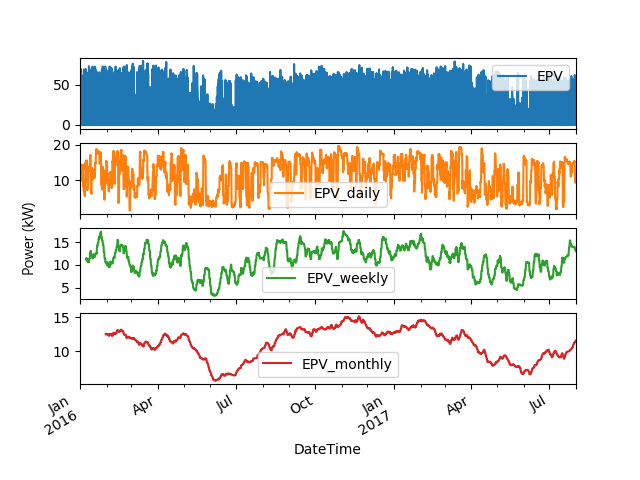
\includegraphics[width=0.5\textwidth]{PV_new.png}
	\centering
	\caption{PV production and its daily, weekly and monthly rolling average.}
	\label{fig:PV}
\end{figure}

\begin{figure}[t]
	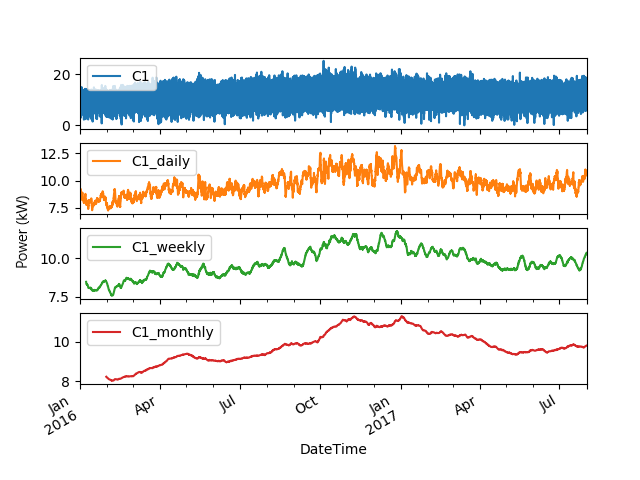
\includegraphics[width=0.5\textwidth]{Load_new.png}
	\centering
	\caption{Electrical load and its daily, weekly and monthly rolling average.}
	\label{fig:load}
\end{figure}

In an off grid-microgrid setting, the optimal size of the components depends heavily on the control policy applied. When the capacity of the installed components is large, a myopic policy can be as good as a look-ahead policy. On the other hand, a good policy that is able to anticipate changes and to act accordingly allows for the reduction of the components size and subsequently the installation cost.

The search for a good policy becomes much more relevant when the size of the components is constraining the operation of the microgrid. Therefore, in this paper we consider a reduced installation for which the applied control policy really impacts the cost of operation for the microgrid. The parameters used for the microgrid configuration in this paper are given in Table \ref{input_param}.

Additionally, the effect of different policies depend on the seasonality of solar irradiation and demand being observed. For instance, during the summer period (November through March in the case of Bolivia) there are high solar irradiation levels that can be used to charge fully the battery most of the days. During this period a myopic rule-based strategy has very similar outcomes with a look-ahead strategy. However, during the winter period (April to October), when solar irradiation is limited and the battery may not be fully charged, a more elaborate strategy is necessary in order to guarantee low-cost security of supply in the microgrid.



%The parameters used for this specific microgrid configuration are given in Table \ref{input_param}. It is important to note that the minimum stable generation level is rather high due to local regulations: the very low diesel price is due to a state subsidy, but the state restricts the operation of all the conventional generators below 80\% of their nominal capacity in order to operate close to the optimal efficiency. This restriction imposes a large discontinuity in the microgrid operation and is further discussed in the results section.

\begin{table}
	\begin{center}
		\renewcommand\arraystretch{1}
		\caption{Input parameters.}
		\begin{tabular}[b]{l r r}
			\hline
			$\maxcharge$ & 120 & kWh \\
			$\chargerate$, $\dischargerate$ & 100 & kW \\
			\chargeEfficienty, \dischargeEfficienty & 75\footnote{The relatively values considered for the charging and discharging are attributed to the technology of the lead-acid batteries.} \% \\ 
			$\OPprice{fuel}$ & 1 & \texteuro/kWh\\
			$\OPprice{curt}$ & 1.5 & \texteuro/kWh \\
			$\OPprice{shed}$ & 10 & \texteuro/kWh \\
			$\OPduration$ & 1 & h\\
			$\overline{\nonSteerable}$ & 120 & kW \\
			$\overline{\steerable}$ & 9 & kW \\
			$\underline{\steerable}$ & 0 & kW \\
			\hline
		\end{tabular}
		\label{input_param}
	\end{center}
\end{table}

	\subsection{Partial Observability}
	    As described in Section~\ref{sec: Simulator}, the process under consideration is non-stationary. The stochastic component of the transition kernel is known to be non-Markovian and the optimal decision requires knowledge of the next $l$ time steps. In supervised learning problems this issue is commonly addressed by state-based networks \cite{taylor2018forecasting}. However, in this paper we take a similar approach as the one considered in the optimization-based controller (Section \ref{sec: optcontroller}). We use the model $M_\psi$ as a 1-step forecaster. After a number of warm-up iterations $B$, we use the model to produce a forecast of the state in the $l$ following time-steps. This forecast is used to augment the actual state which is used to train the controller. A critical assumption of our approach is that the gradual changes to the system dynamics are sufficiently smooth for a single model $M_\psi$ to successfully track these changes.

	\subsection{Action Space and Meta-Actions}
	
%	The action space should describe the controllability of the system. In the case of the microgrid controller, the agent can only decide how much energy shall be release in the system, and from which source. We model this as a vector of $a = (c,x)$ where $c$ is the index of the controlled item and $x$ the magnitude of the control. In the microgrid setting the possible items are the generator and the batteries. A magnitude for the battery describe how much discharge, while the magnitude for the generator describes how much energy to produce.
%
%	It occurs to the author to describe the action space as 1 dimensional, but we found this to work better in practice.
%	The action space visited by the optimal controller from Section~\ref{sec: optcontroller} in Figure~\ref{fig:action_space} is constrained to a subspace of $\mathbb{R}^2$, and aside the action space visited by our algorithm ~\ref{fig:action_space_ppo}.
%

	Due to the continuous and high-dimensional nature of the state and the action spaces of the problem, reinforcement learning methods cannot be applied in their exact form. However, recent developments in the field of reinforcement learning have made possible the design of approximate optimal policies using function approximation.

	In our setting, function approximation alone does not suffice. The action space visited by the optimal controller from Section~\ref{sec: optcontroller} is constrained to a subspace of $\mathbb{R}^2$. Therefore, we elaborate on the design of a small and discrete set of actions $A'$ that maps to the original action space $A$.  This step is necessary for the use of policy-based algorithms, as the maximization problem defined in \eqref{eqn: optimalpolicy} is hard to solve.
	
	The meta-action $a'_{t}$ for each decision step $t$ is defined as: $$a'_{t} \in A'= \left\lbrace ``C",``D", ``G" \right\rbrace.$$ 
	
	Meta-action $``C"$ indicates the action to charge energy in the battery, when there is excessive renewable production ($\Delta P_t > 0 $). With meta-action $``D"$ we select to prioritize the discharge of the battery for covering the deficit of energy ($\Delta P_t < 0 $) in the microgrid. In case the battery does not suffice for covering this deficit, the generator will be activated. Alternatively, meta-action $``G"$ is used to prioritize the generator for supplying the deficit of energy and the battery will be discharged only in the case that the maximum generating limit ($\overline{\steerable}$) is reached.
	
	%Each of the storage devices can have status $y_{b,t}\in Y$ of charging, discharging or idling where $Y= \left\lbrace ``C",``D", ``I" \right\rbrace $. We define a discrete action $a'_{t} \in A'$ that can take values from all the possible combinations of $y_{b,t}$ as:
	%\begin{gather}
	%a'_{t} = (y_{b,t}, \forall b \in \mathbb{B}) \in Y^{|B|}
	%\end{gather}
		

	In particular, at each decision step $t$ we provide as inputs to the dispatch Algorithm \ref{algoRBC}, the observed residual generation $\Delta P_t$ and the meta-action $y_t=a'_t$. The residual generation $\Delta P_t$ is computed after the realization of the stochastic variables ($\nonSteerable_t$, $\nonFlexible_{t}$) as $\Delta P_t = \nonSteerable_t - \nonFlexible_{t}$.

    Defining the action space in this way allows the use of the dispatch rule defined in Algorithm \ref{algoRBC} to obtain the control actions $a_t = (\charge_{t}, \discharge_{t}, \steer_{t})$. The discrete action space $A'$ simplifies the problem but restricts the class of possible policies, which sometimes harms the performance of the reinforcement learning methods.	We leave the problem of directly optimizing continuous actions as future work.
	
	%Preliminary experiments with the continuous action space $A$ were unsuccessful

	

%\begin{figure}[t]
%	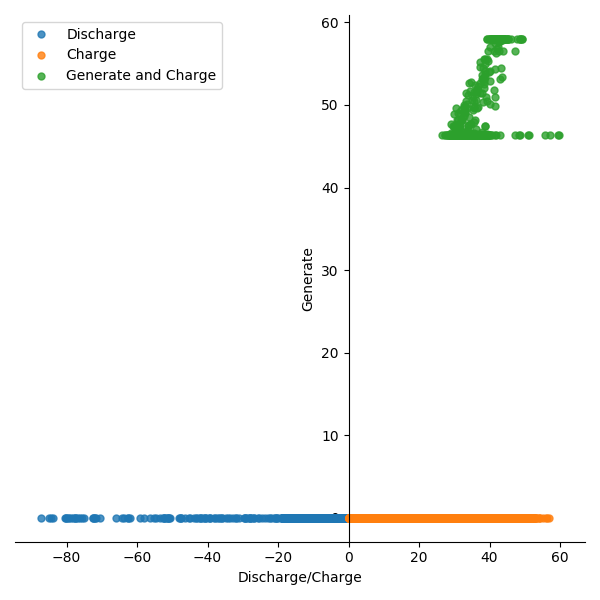
\includegraphics[width=0.4\textwidth]{action_space.png}
%	\centering
%	\caption{Action space covered by the optimization-based controller.}
%	\label{fig:action-space}
%\end{figure}

\subsection{Comparison with the benchmarks}
% rule basd
% mpc + 1h (~ model based)
% model-free
% model based

The algorithm is compared against the two benchmarks described in Section \ref{sec: Simulator} and the simple model-free version of PPO \cite{Schulman2017}. An optimization controller with perfect knowledge and 1 period of look-ahead (``MPC-1") is considered in order to obtain a fair comparison to the proposed algorithm. An optimization controller with 24 periods of look-ahead and perfect knowledge (``MPC-24") is used to provide an upper bound on the performance of any control strategy. Additionally, a myopic rule-based controller, indicated in the results as ``heuristic", is used to provide a lower bound. We use PPO to denote the baseline algorithm which only performs model-free updates and \textsc{D-Dyna} to denote our method.

The label ``training step" on the x-axis refers to the number of times a new set of trajectories has been used for computing one or multiple gradient steps. For a fair comparison we fix the total number of samples available for the agent and compute the number of samples per training update accounting for the number of gradient step and the number of planning steps. Finally, results are averaged for 10 random seeds in order to account for stochasticity.
	    
        
\subsection{Generalization}
% explain what is generalization
% how you test generalization and why
% show and discuss results


One of the challenges of real world applications is the occurrence of changes in the transition dynamics. As described in Section \ref{sec: Simulator}, the dynamics of the microgrid are composed of a deterministic part and a stochastic part. The stochastic part is not controllable and therefore constitutes a source of progressive change. 

In this section, we evaluate the ability of model-based algorithm to adapt to gradual changes that occur in the state space. An algorithm that generalizes over unseen data distributions can provide a good initialization for fine-tuning the new controller.
The following protocol was used for training and evaluation of the proposed algorithms. We split the original dataset in a training set and a test set: the training set ranges from January 2016 to December 2016, while the test set ranges from January 2017 to July 2017. 

\textcolor{black}{Figure~\ref{fig:rl-results} presents the cumulative returns (costs) collected in the test set by the compared algorithms as a function of the training progress (i.e. training steps). In other words, at each training step performed by the RL algorithms we perform an evaluation of all considered algorithms in the test set. We observe that the reinforcement learning methods approximately yield a 25\% cost reduction in comparison to the rule-based controller and the model-based method is comparable to the upper bound set by MPC-24}. As illustrated in Figure~\ref{fig:rl-results}, introducing a model benefits generalization and both the baseline and the proposed algorithm are able to outperform the heuristic. We conjecture that using artificially generated states accelerates the learning process and provides a wider coverage of the state (exploration) and action space manifold, resulting in better generalization properties. 

Additionally, we observe that the proposed model-based method is able to outperform the ``MPC-1" benchmark. We can argue that the obtained policy manages to resemble a look-ahead policy that takes optimal actions with respect to several steps ahead. This outcome is rather valuable because by using such a policy we can reduce the investment cost for equipment (e.g. battery capacity or diesel generators), without jeopardising the security of supply in the microgrid. \textcolor{black}{Additionally, the cost reduction achieved by the proposed algorithm mainly implies a reduction in the use of the diesel generator and the higher utilization of RES. This effect subsequently results in an overall reduction of CO$_2$ emissions and promotes sustainable energy utilization in the context of rural electrification.}

\begin{figure}[t]
	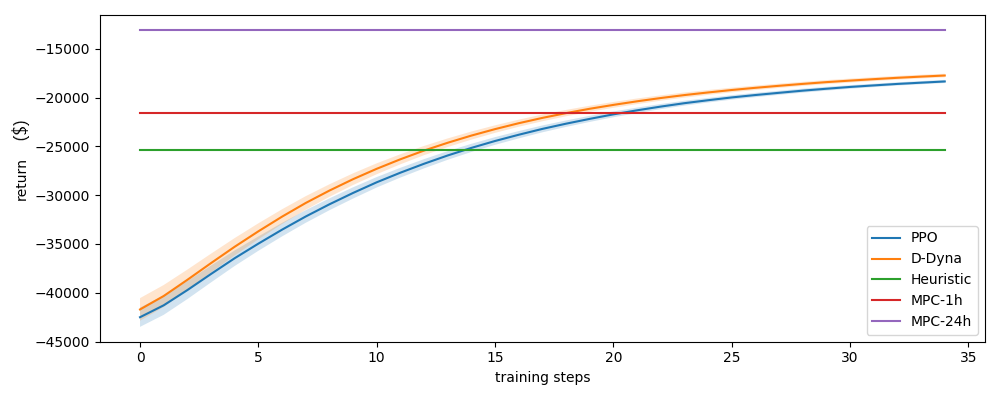
\includegraphics[width=0.51\textwidth]{MicroGrid-Long-v0.png}
	\centering
	\caption{Cumulative returns (cost) on the test set as a function of the training progress of the RL algorithms.}
	\label{fig:rl-results}
\end{figure}

\subsection{Robustness} \label{sec: robustness}

In this section, we evaluate the performance of the proposed model-based algorithm in sudden changes as defined in Section~\ref{sec: Simulator}. An example of such a change is the abrupt failure of the storage system, where the battery capacity is suddenly unavailable. 

We simulate this change in the following way. Let $x_{t}$ be the random discrete variable taking at each time-step the value 0 if the battery has failed and the value 1 if the battery is still operational. We assume that $x_{t}$ follows a Bernoulli probability distribution where $Pr(x_{t}=1)=p_{t}$, with $p_{t}$ following a linear decay in time and $p_{0}= 0.99$. If the battery fails, then the maximum storage capacity is considered to be reduced to zero ($\maxcharge=0 $ kWh). After a failure, it is assumed that the battery equipment is fixed and the storage capacity is restored to its initial value in a period of $N=370$ hours. Failures can occur during both training and testing.

For this experiment, we have increased the size of the generator at a level that covers the entire demand. In this way, we want to evaluate the capability of the proposed model-based method to switch from a regime where, the battery is mainly used when it is available, to only using the generator in the event of a battery failure.

Under this scenario, we evaluate the benchmark controllers, the model-free method as well as the model-based method. As we can see in Figure~\ref{fig:change}, all benchmarks perform poorly while the proposed algorithm is able to quickly adapt to the new drastically changing dynamics. The poor performance of the benchmark controllers is justified by the fact that there is no special equipment for the detection of the failure. The superiority of the proposed model-based algorithm stems from its ability to detect the change since the model has been exposed to similar incidents during training.

    
    \begin{figure}[t]
    	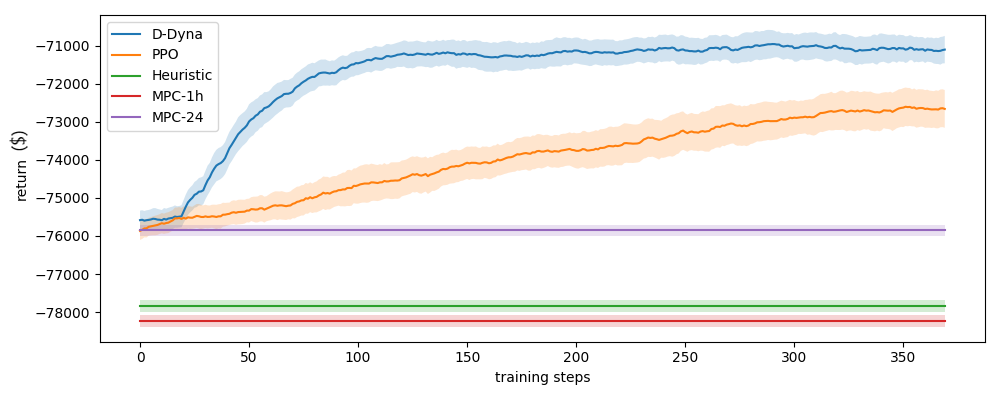
\includegraphics[width=0.51\textwidth]{robustness.png}
    	\centering
    	\caption{Cumulative returns (costs) when the battery is excluded as a function of the training progress of the RL algorithms.}
		\label{fig:change}
    \end{figure}
    

\subsection{Transfer}

    In Reinforcement Learning, transfer learning is the ability of speeding up learning on new MDPs by reusing past experiences between similar MDPs. For real world applications, it would be desirable to obtain an algorithm that has the ability to learn off-line and adapt as the task changes. 

    A natural instance of such feature is to consider each month as a separate MDP and evaluate the ability to transfer knowledge across months. Note that each month has a different distribution of the stochastic component of the transition kernel.
    
	We set up the following experimental protocol. We use January 2016 to pre-train the algorithms. Then we initiate the training process for February and August 2016 using the pre-trained model. Intuitively transfer should be easier if the data distributions are close in time, and harder otherwise.
	
    The results of the described protocol are presented in Figures~\ref{fig:transfer-feb} and~\ref{fig:transfer-aug}. As we can see, transferring the model and the control allows for better performance than learning from scratch. As illustrated, the model-based method can substantially speed up the learning process. The proposed method is shown to slightly outperform the ``heuristic" as well as the ``MPC-1h" benchmarks. However, in August the results are much better in that the model-based method is approaching the performance of the ``MPC-24h" policy, while the rest of the benchmarks are falling behind. 
    
    As discussed in Section \ref{sec: config}, the effect of different policies depends on the period of the year. We can observe that the results in February are substantially different in comparison to August. There is a small discrepancy between the returns from the myopic and the optimization-based controller with perfect knowledge during February. On the other hand, during August the two policies show an increased difference in returns. 


    \begin{figure}
     	\centering
     	\begin{minipage}{0.5\textwidth}
     		\centering
     		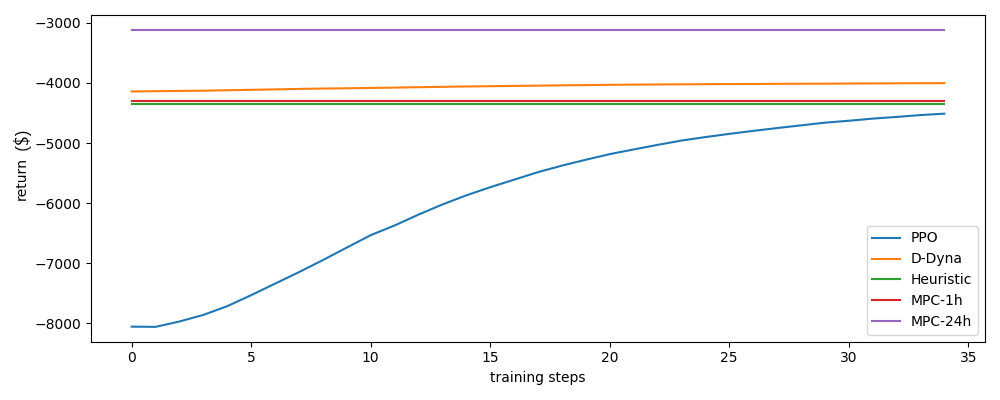
\includegraphics[width=1.05\textwidth]{MicroGrid-Feb-v0.png}
     		\caption{Cumulative returns (cost) during February as a function of the training progress of the RL algorithms.}
			\label{fig:transfer-feb}
     	\end{minipage} \hfill
     	\begin{minipage}{0.5\textwidth}
     		\centering
     		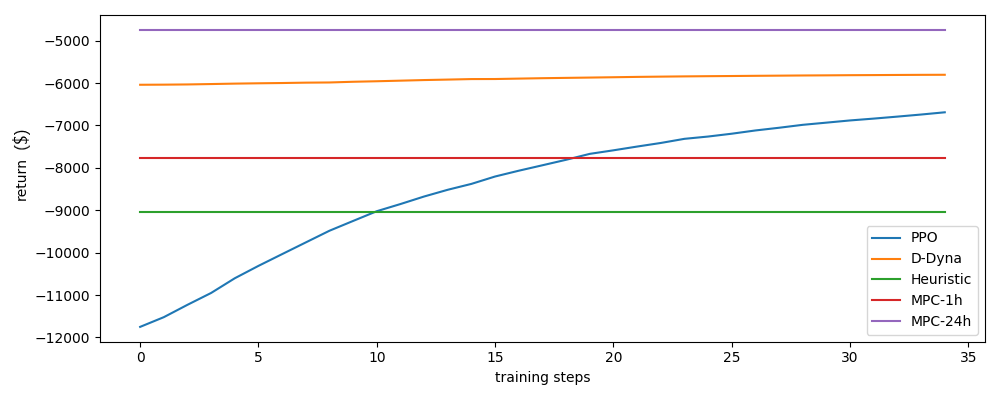
\includegraphics[width=1.05\textwidth]{MicroGrid-Aug-v0.png}
     		\caption{Cumulative returns (cost) during August as a function of the training progress of the RL algorithms.}
			\label{fig:transfer-aug}
     	\end{minipage}
     
     \end{figure}

\section{Conclusions} \label{sec: conclusions}
    In this paper, a novel model-based reinforcement learning algorithm is proposed for the lifelong control of a microgrid. First, an open-source reinforcement framework for the modeling of an off-grid microgrid for rural electrification is presented. The control problem of an isolated microgrid is casted as a Markov Decision Process (MDP). The proposed algorithm learns a model online using the collected experiences. This model is used to sample states during the evaluation step of the proximal policy optimization (PPO) algorithm.
    
    We compare the proposed algorithm to the standard benchmarks in the literature. Firstly, a rule-based control that takes decisions in a myopic manner based only on current information and secondly an optimization-based controller with look-ahead are considered for comparison purposes.
    
    We evaluate the generalization capabilities of the proposed algorithm by comparing its performance in out-of-sample data to the benchmarks. It is found that the use of the model to create artificial states leads to improved exploration and superior performance compared to the myopic rule-based controller and the MPC with one step look-ahead.
    
    We evaluate the robustness of the proposed algorithm when being subject to sudden changes in the transition dynamics, such as equipment failure. The results indicate that the model-based method has the ability to adapt rapidly to severe changes in contrast to the benchmarks that are unable to detect changes and perform poorly to the subjected task.
    
    Finally, we evaluate the ability to transfer knowledge from one training session to the next. The results show large gains in computational time when initiating training on a new dataset with a pre-trained model.

	One important conclusion is that the proposed model-based reinforcement learning method is able to adapt to changes, both gradual and abrupt. Overall, the proposed method succeeds in tackling the key challenges encountered in the lifelong control of an off-grid microgrid for rural electrification. Future work should be directed to the design of a low dimensional continuous action space in order to be able to obtain results similar to the optimization-based controller.
    
	In future work, we plan to perform experiments directly with continuous actions. As explained in the paper, discretizing the actions makes reinforcement learning and exploration much faster, but introduces approximation errors that may account for the slightly worse performance of reinforcement learning in some settings. Since actions are concentrated to restricted areas of the joint action space, we believe that it is necessary to impose constraints on the continuous actions during learning. \textcolor{black}{Additionally, future work could be directed towards incorporating the effect of efficiency improvement on the microgrid components. For instance,  improvements in the efficiency of consumer appliances are expected to progressively decrease the average demand profile. On the other hand, improvements in the efficiency of solar PV or in storage systems due to technological improvements are expected to have an impact on the control policy.}

\section{Acknowledgements}
This research is carried out in the framework of the project Dynamically Evolving Long-Term Autonomy (DELTA), a European research project funded under the CHIST-ERA scheme (\url{http://www.chistera.eu/}). Anders Jonsson is partially supported by the grants TIN2015-67959 and PCIN-2017-082 of the Spanish Ministry of Science. The authors would like to thank Sergio Balderrama for the provision of measured data from the ''El Espino" microgrid in Bolivia and Alessandro Davide Ialongo for the fruitful discussion.


% In the unusual situation where you want a paper to appear in the
% references without citing it in the main text, use \nocite
% \nocite{langley00}

\bibliography{reference.bib}
\bibliographystyle{src/icml2020}

\section*{Appendix}


\begin{algorithm}[t]
	\caption{Power dispatch.}
	\begin{algorithmic}[1]
		\STATE \textbf{Inputs:} $\Delta P_t$ , $y_t$, $\chargerate$, $\dischargerate$, $\overline{\steerable}$
		\STATE \textbf{Initialize:}$\discharge_t \gets 0$,$\charge_t\gets 0$,  $\steer_t\gets 0$
		\IF{ $\Delta P_t \geq 0 $}
		\IF{ $y_t = ``C" $}
		\STATE $\charge_t = \min(P^{RES},\chargerate)$ 
		\ENDIF
		\STATE $\Delta P_t \leftarrow \Delta P_t - \charge_t$
		\ELSE
		\IF{ $y_t = ``D" $}
		\STATE $\discharge_t = \min(-P^{RES},\dischargerate)$ 
		\STATE $\Delta P_t \leftarrow \Delta P_t +\discharge_t$
		\STATE $\steer_t=\min(-P^{RES},\overline{\steerable})$ 
		\ENDIF
		\IF{ $y_t = ``G" $}
		\STATE $\steer_t=\min(-P^{RES},\overline{\steerable})$ 
		\STATE $\Delta P_t \leftarrow \Delta P_t + \steer_t$
		\STATE $\discharge_t = \min(-P^{RES},\dischargerate)$ 
		\ENDIF
		\ENDIF
	\STATE \textbf{Output:} $a_t$
	\end{algorithmic}
	\label{algoRBC}
\end{algorithm}



\begin{algorithm}[t]
	\caption{Model-predictive controller.}
	\begin{algorithmic}[1]
		\STATE \textbf{Inputs:} $N$, $\OPprice{curt}$ , $\OPprice{shed}$, $\OPprice{fuel}$,$F_1$, $F_2$, $\chargeEfficienty$, $\dischargeEfficienty$, \\
		$\chargerate$, $\dischargerate$, $\maxcharge$, $\overline{\steerable}$ , $\underline{\steerable}$, $\widehat{\nonFlexible}_{t}$,$\widehat{\nonSteerable_{t}}$
		\STATE \textbf{Solve:}
		\begin{align}
	\hspace{-12pt}	\min &  \sum_{k=0}^{N} \OPduration \big(\OPcost{fuel}_t + \OPcost{curt}_t + \OPcost{shed}_t \big)&&& \nonumber\\
	\hspace{-12pt}s.t. & \forall k \in \{0,...,N-1 \}: \nonumber \\
	    & \widehat{\nonSteerable_{t+k}} + \steer_{t+k} + \discharge_{t+k} + \shed_{t+k}=&&\nonumber\\
        &\hspace{0pt}\charge_{t+k} + \curtail_{t+k}  + \widehat{\nonFlexible}_{t+k} \hspace{28pt} &&\nonumber\\
        &\OPcost{curt}_{t+k} = \curtail_{t+k} \cdot \OPprice{curt} \hspace{38pt} &&\nonumber\\
        &\OPcost{shed}_{t+k} = \shed_{t+k} \cdot \OPprice{shed} \hspace{35pt}&&\nonumber\\
        &\OPcost{fuel}_{t+k} = F_{t+k} \cdot \OPprice{fuel} \hspace{38pt}&&\nonumber\\
        &F_{t+k} = F_1 + F_2 \cdot \steer_{t+k} \hspace{20pt}&&\nonumber\\
        &SoC_{t+k+1} = SoC_{t+k}+ \Delta t  \cdot(\chargeEfficienty \charge_{t+k} -  \frac{\discharge_{t+k}}{\dischargeEfficienty}) \hspace{40pt}&\nonumber\\
        &SoC_{t+k}, \charge_{t+k}, \discharge_{t+k} \geq 0 \hspace{5pt}&&\nonumber\\
        &\charge_{t+k} \leq \chargerate \hspace{75pt}&&\nonumber\\
        &\discharge_{t+k} \leq \dischargerate \hspace{75pt} &&\nonumber\\
        &SoC_{t+k} \leq \maxcharge \hspace{64pt} &&\nonumber\\
        &\steer_{t+k} \leq \overline{\steerable} \cdot n_{t+k} \hspace{38pt} &&\nonumber\\
        &\steer_{t+k} \geq \underline{\steerable} \cdot n_{t+k}  \hspace{38pt} &&\nonumber\\
        &n_{t+k} \in \{0, 1\}  \hspace{62pt} &&\nonumber
		\end{align}
	\STATE \textbf{Output:} $a^{N}_t$
	\end{algorithmic}
	\label{mpc}
\end{algorithm}

% \subsection*{Notation}
% \subsection*{\textit{\textbf{Set and indices}}}

% \begin{itemize}
% 	\item $t$, decision time step
% 	\item $k$, look-ahead step
% 	\item $\mathcal{A}$, action space
% 	\item $\mathcal{A'}$, meta-action space
% 	\item $\mathcal{S}$, state space
% \end{itemize}  

% \vspace*{0.25cm}
% \subsection*{\textit{\textbf{Parameters}}}
% \begin{itemize}
%     \item $F_1$, $F_2$, fuel consumption parameters
%     \item $N$, number of look-ahead periods
%     \item $\widehat{\nonFlexible}$, load forecast (kW)
% 	\item $\chargerate$, $\dischargerate$, maximum charge and discharge rate (kW)
% 	\item $\overline{\nonSteerable}$, non steerable generation (kW)
% 	\item $\overline{\steerable}$, steerable generator capacity (kW)
% 	\item $\underline{\steerable}$, minimum steerable generation (kW)
% 	\item $\maxcharge$, $\mincharge$, maximum and minimum battery capacity (kWh)
% 	\item $\widehat{\nonSteerable}$, renewable generation forecast (kW)
% 	\item $\OPduration$, simulation and control period duration (h)
% 	\item $\chargeEfficienty$, $\dischargeEfficienty$, charge and discharge efficiency (\%) 
% 	\item $\OPprice{curt}$, curtailment price (\texteuro/kWh)
% 	\item $\OPprice{fuel}$, fuel price (\texteuro/kWh)
% 	\item $\OPprice{shed}$, load shedding price (\texteuro/kWh)
% \end{itemize}
% \subsection*{\textit{\textbf{Variables}}}
% \begin{itemize}
% 	\item $a$, control actions vector
% 	\item $a'$, meta-actions vector
% 	\item $\nonFlexible$, non-flexible load (kW)
% 	\item $\OPcost{fuel}$, fuel cost (\texteuro)
% 	\item $\OPcost{curt}$, curtailment cost (\texteuro)
% 	\item $\OPcost{shed}$, lost load cost (\texteuro)
% 	\item $F_t$, fuel consumption ($l$)
% 	\item $k$, binary variable 
% 	\item $n_t$, number of cycles of the battery
% 	\item $\charge$, $\discharge$, charging and discharging power (kW)
% 	\item $\shed$, load shed (kW)
% 	\item $\curtail$, generation curtailed (kW)
% 	\item $\steer$, generation activated (kW)
% 	\item $\nonSteerable$, renewable generation (kW)
% 	\item $\charge$, charged energy of battery (kWh)
% 	\item $\discharge$, discharged energy of battery (kWh)
% 	\item $SoC$, state of charge of battery (kWh)
% 	\item $s$, control state vector 
% 	\item $\bar{s}$, stochastic state vector
% 	\item $\ubar{s}$, deterministic state vector
% 	\item $y_t$, discrete decision about the use of the equipment
% 	\item $\Delta P_t$, residual generation level (kW)
% \end{itemize}

% \subsection*{\textit{\textbf{Functions}}}
% \begin{itemize}
% 	\item $P^{C}_{t}(\cdot)$, load probability distribution
% 	\item $P^{\nonSteerable}_{t}(\cdot)$, renewable generation probability distribution
% 	\item $s(\cdot)$, storage capacity as a function of the number of cycles
% \end{itemize}
\end{document}


% This document was modified from the file originally made available by
% Pat Langley and Andrea Danyluk for ICML-2K. This version was created
% by Iain Murray in 2018, and modified by Alexandre Bouchard in
% 2019 and 2020. Previous contributors include Dan Roy, Lise Getoor and Tobias
% Scheffer, which was slightly modified from the 2010 version by
% Thorsten Joachims & Johannes Fuernkranz, slightly modified from the
% 2009 version by Kiri Wagstaff and Sam Roweis's 2008 version, which is
% slightly modified from Prasad Tadepalli's 2007 version which is a
% lightly changed version of the previous year's version by Andrew
% Moore, which was in turn edited from those of Kristian Kersting and
% Codrina Lauth. Alex Smola contributed to the algorithmic style files.

